\begin{figure}[!htbp]
\centering
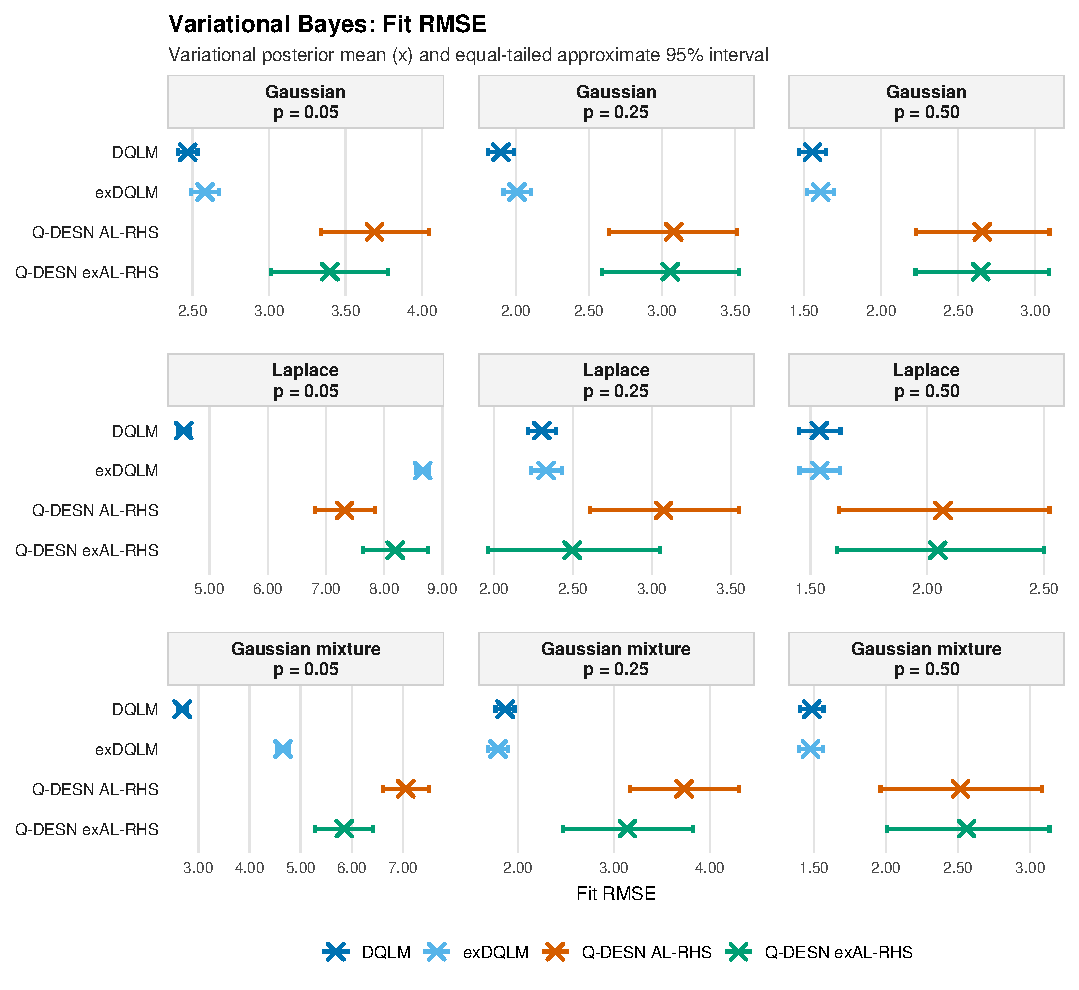
\includegraphics[width=0.98\textwidth]{figures/independent_simulation/qdesn_validation_500obs_vb_fit_rmse_intervals.pdf}
\caption{Variational Bayes posterior uncertainty for fit rmse in the single-quantile simulation study. Horizontal segments show equal-tailed approximate 95\% variational posterior intervals; crosses mark posterior means. Each panel uses its own horizontal scale, and lower values are better. Bands condition on the fixed simulated data set, evaluation grid, and case-specific model specification.}
\label{fig:simulation-500obs-vb-fit_rmse-intervals}
\end{figure}

\begin{figure}[!htbp]
\centering
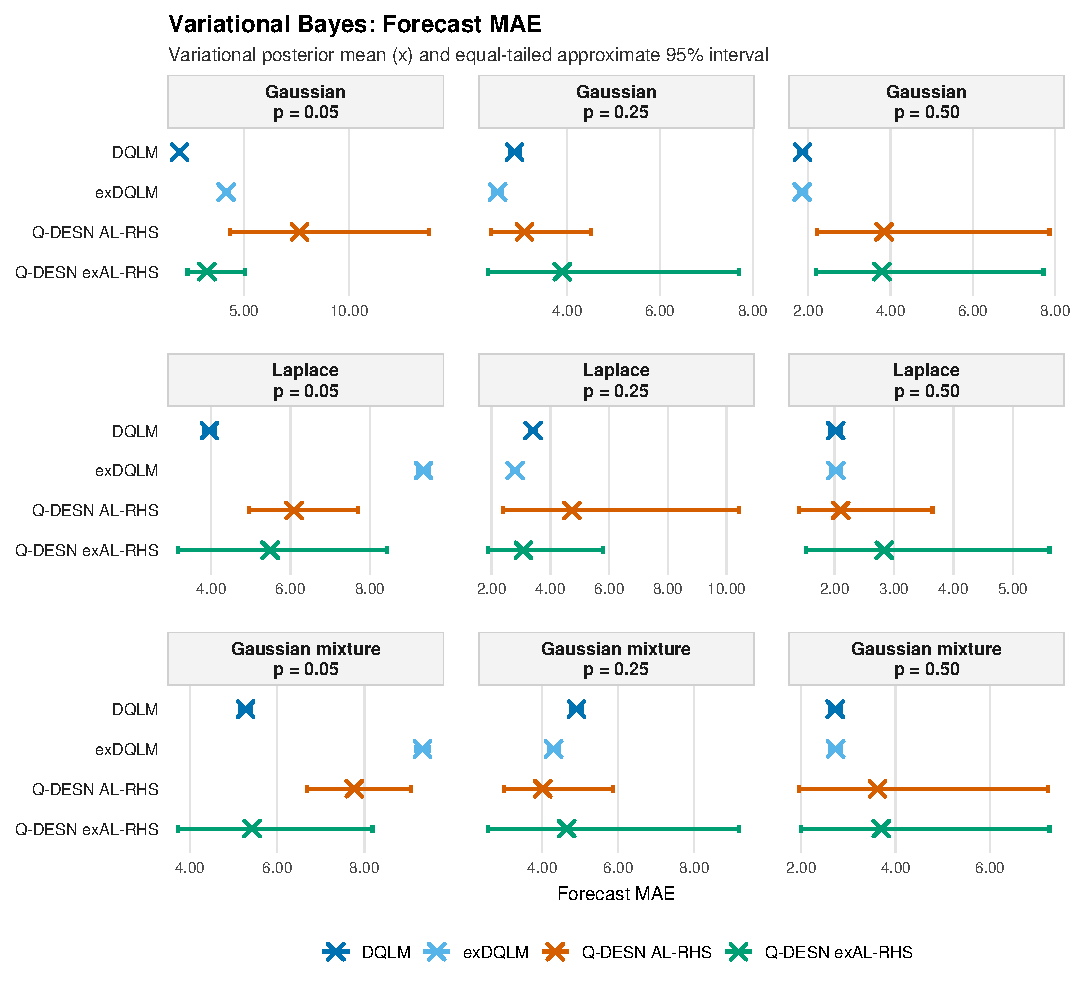
\includegraphics[width=0.98\textwidth]{figures/independent_simulation/qdesn_validation_500obs_vb_forecast_mae_intervals.pdf}
\caption{Variational Bayes posterior uncertainty for forecast mae in the single-quantile simulation study. Horizontal segments show equal-tailed approximate 95\% variational posterior intervals; crosses mark posterior means. Each panel uses its own horizontal scale, and lower values are better. Bands condition on the fixed simulated data set, evaluation grid, and case-specific model specification.}
\label{fig:simulation-500obs-vb-forecast_mae-intervals}
\end{figure}

\begin{figure}[!htbp]
\centering
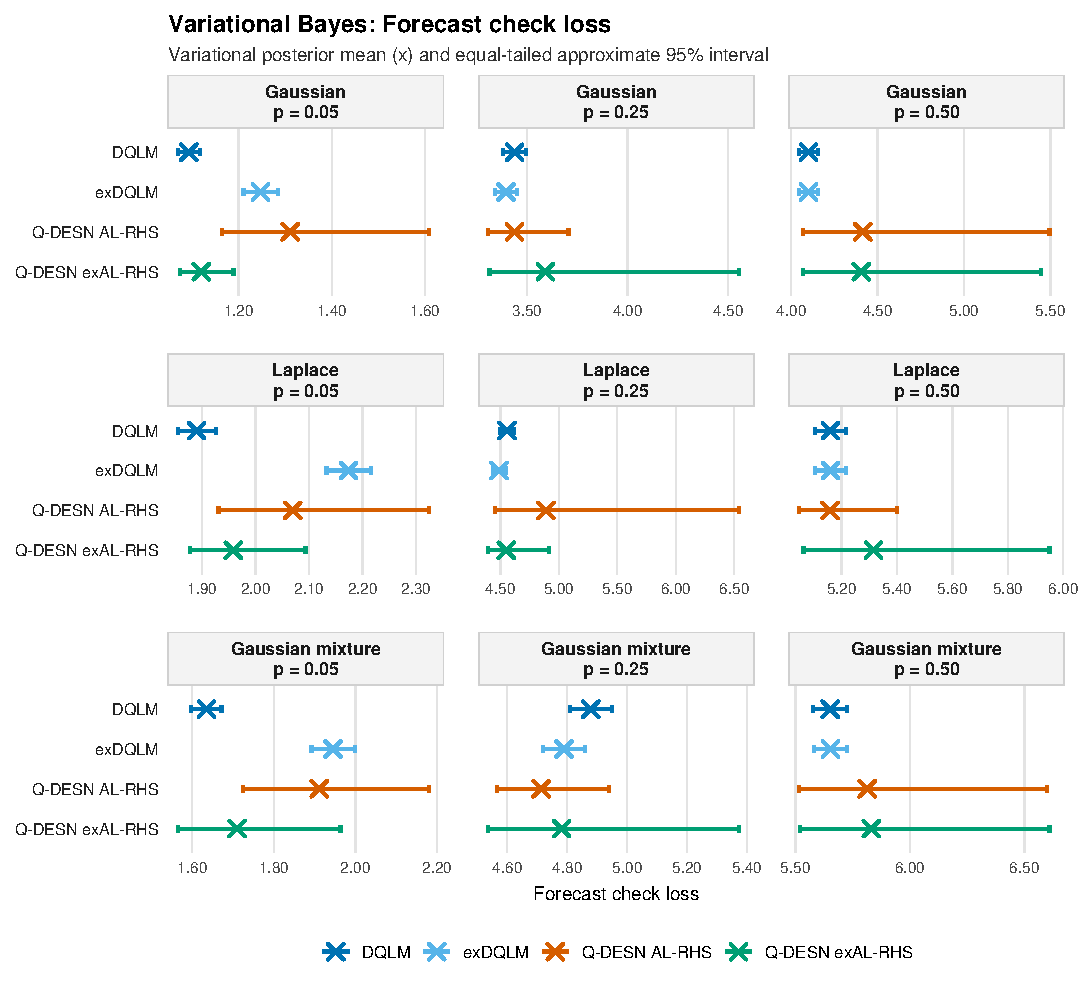
\includegraphics[width=0.98\textwidth]{figures/independent_simulation/qdesn_validation_500obs_vb_forecast_check_loss_intervals.pdf}
\caption{Variational Bayes posterior uncertainty for forecast check loss in the single-quantile simulation study. Horizontal segments show equal-tailed approximate 95\% variational posterior intervals; crosses mark posterior means. Each panel uses its own horizontal scale, and lower values are better. Bands condition on the fixed simulated data set, evaluation grid, and case-specific model specification.}
\label{fig:simulation-500obs-vb-forecast_check_loss-intervals}
\end{figure}
